% !TEX program = pdflatex
\documentclass[10pt,aspectratio=169,table]{beamer}
\usepackage[UTF8]{ctex}
\usepackage{graphicx}
\usepackage{hyperref}
\usepackage{booktabs}
\usepackage{tikz}
\usepackage{xcolor}

\usetheme{Madrid}
\definecolor{sysublue}{RGB}{0,51,102}
\definecolor{sysured}{RGB}{180,30,30}
\definecolor{phase2color}{RGB}{237,125,49}
\definecolor{mygreen}{RGB}{0,128,0}
\setbeamercolor{structure}{fg=sysublue}
\setbeamercolor{title}{fg=white,bg=sysublue}
\setbeamercolor{frametitle}{fg=white,bg=sysublue}
\setbeamercolor{block title}{fg=white,bg=sysublue}
\setbeamercolor{block body}{bg=sysublue!5}
\setbeamertemplate{footline}[frame number]
\setbeamertemplate{navigation symbols}{}
\setbeamerfont{frametitle}{size=\large}
\setbeamerfont{block title}{size=\small}
\setbeamerfont{block body}{size=\footnotesize}

\title[电路原理图 OCR]{基于 PaddleOCR-VL 的电路原理图 OCR 研究与实现}
\subtitle{数据集构建 · 模型训练 · 多维度评估}
\author[张健宁]{\textbf{张健宁}}
\institute[中山大学]{中山大学}
\date{2026年7月20日}

\begin{document}

\begin{frame}[plain]
  \titlepage
  \begin{center}
    \footnotesize \url{https://github.com/ZhangJ83/circuit-ocr-paddle}
  \end{center}
\end{frame}

\begin{frame}{目录}
  \tableofcontents
\end{frame}

% ═══════════ 引言 ═══════════
\section{引言}

\begin{frame}{项目背景与动机}
  \begin{columns}[T]
    \column{0.5\textwidth}
      \begin{block}{电路原理图 OCR 的挑战}
        \footnotesize
        \begin{itemize}
          \item 电路图含有密集的工程文字：元件标号、参数值、引脚号、网络标签
          \item 现有 OCR 引擎（PaddleOCR、Tesseract、EasyOCR）均无法处理
          \item 基座 VLM 输出为幻觉文本，CompF1=0, LineAcc=0
          \item 小数据集上微调存在严重的模态塌缩问题
        \end{itemize}
      \end{block}
    \column{0.5\textwidth}
      \begin{block}{本项目工作}
        \footnotesize
        \begin{enumerate}
          \item 构建电路原理图 OCR 标注数据集（7 轮验证）
          \item 提出合成文字数据防塌缩策略
          \item Phase 1-4 共 8 组系统消融实验
          \item 全开源：代码、数据、权重、报告、Demo
        \end{enumerate}
      \end{block}
  \end{columns}
\end{frame}

% ═══════════ 数据集 ═══════════
\section{数据集构建}

\begin{frame}{数据集概览}
  \begin{table}
    \centering
    \footnotesize
    \begin{tabular}{lp{5cm}}
      \toprule
      \textbf{维度} & \textbf{证据} \\
      \midrule
      数据规模 & 1,520 训练 + 150 测试 + 150 验证，4,810 个 OCR 实例 \\
      标注准确性 & 7 轮递进式验证管线，质量报告含 12 组可视化对比 \\
      数据多样性 & KiCad 原理图 + 合成文字图片 + 真实手机拍照 \\
      难度分层 & OCR 实例数 + 文字密度 + 结构复杂度 + 参数值丰富度\\
      \bottomrule
    \end{tabular}
  \end{table}
  \begin{center}
    \footnotesize 数据集仓库：\url{https://github.com/ZhangJ83/circuit_ocr_dataset_final}
  \end{center}
\end{frame}

\begin{frame}{数据规模与来源}
  \begin{columns}[T]
    \column{0.48\textwidth}
      \begin{block}{训练数据构成}
        \footnotesize
        \begin{itemize}
          \item KiCad 原理图：\textbf{1,200} 张（自绘设计，SVG 导出）
          \item 合成文字图片：\textbf{300} 张（PIL 生成，6 种模板）
          \item 真实手机拍照：\textbf{20} 张（打印 A4 后拍摄）
          \item 测试集：150 张，全部为真实 KiCad 电路图
        \end{itemize}
      \end{block}
    \column{0.52\textwidth}
      \begin{center}
        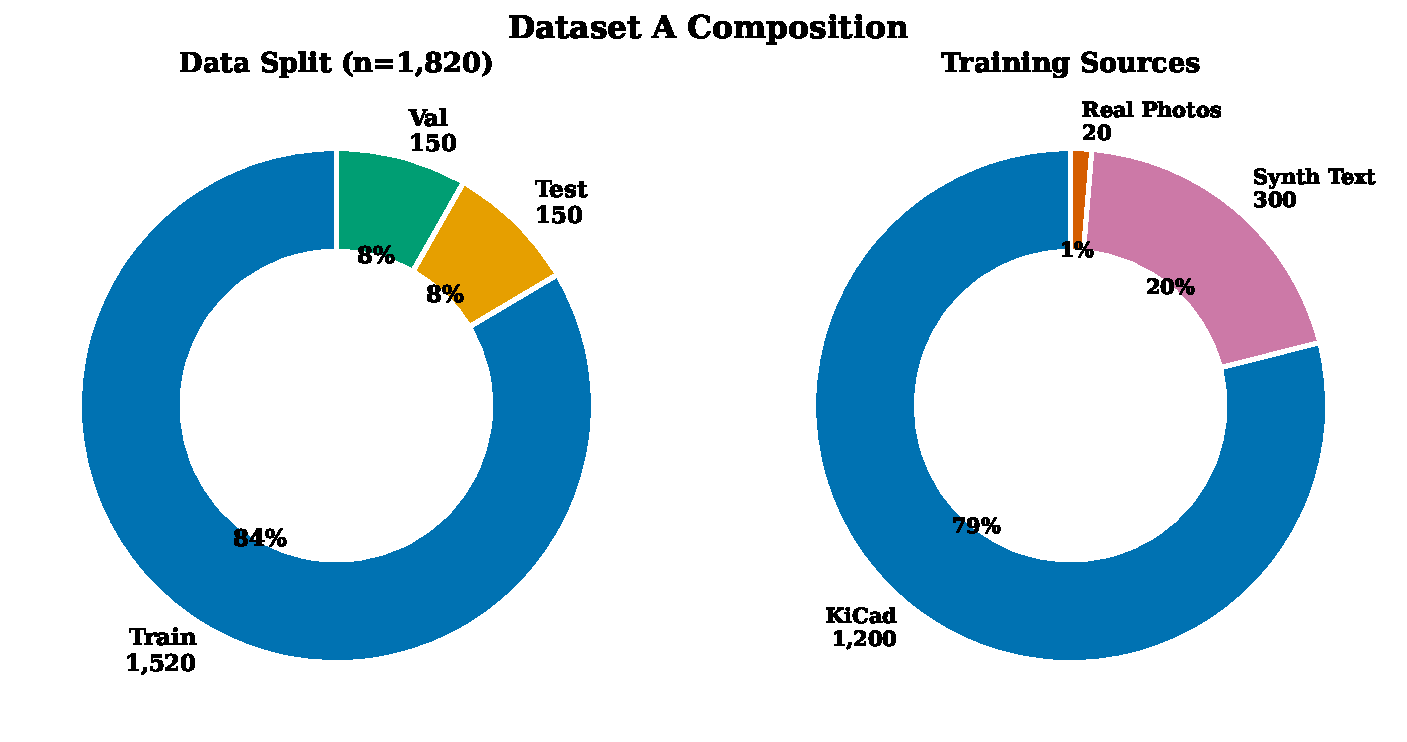
\includegraphics[width=\textwidth]{../slides_figures/dataset_composition.pdf}
      \end{center}
  \end{columns}
\end{frame}

\begin{frame}{标注质量保证}
  \begin{columns}[T]
    \column{0.45\textwidth}
      \begin{block}{7 轮验证管线}
        \footnotesize
        \begin{enumerate}
          \item JSON Schema 自动校验
          \item 图片路径一致性检查
          \item 控制字符扫描过滤
          \item 元件标号正则匹配
          \item 参数值单位标准化
          \item KiCad 网表交叉验证
          \item 人工抽检（10\% 样本）
        \end{enumerate}
      \end{block}
    \column{0.55\textwidth}
      \begin{block}{质量报告}
        \footnotesize
        \begin{itemize}
          \item 量化指标统计完整
          \item 12 组 GT-vs-Image 可视化对比
          \item 多维难度标签体系
        \end{itemize}
      \end{block}
  \end{columns}
\end{frame}

\begin{frame}{数据多样性}
  \begin{columns}[T]
    \column{0.5\textwidth}
      \begin{block}{三种数据来源}
        \footnotesize
        \begin{itemize}
          \item KiCad 矢量导出：统一渲染、矢量线条
          \item 合成文字图：白底黑字、多字号、6 种布局
          \item 真实拍照：自然光照、CMOS 噪声、透视倾斜
        \end{itemize}
      \end{block}
    \column{0.5\textwidth}
      \begin{block}{改进方向}
        \footnotesize
        \begin{itemize}
          \item 真实拍照仅 20 张（1.3\%），量不足
          \item 原理图全为 KiCad 单一来源
          \item 缺少扫描文档、模糊、遮挡样本
          \item 缺少多 EDA 工具导出对比
        \end{itemize}
      \end{block}
  \end{columns}
\end{frame}

\begin{frame}{数据集关键指标一览}
  \begin{center}
    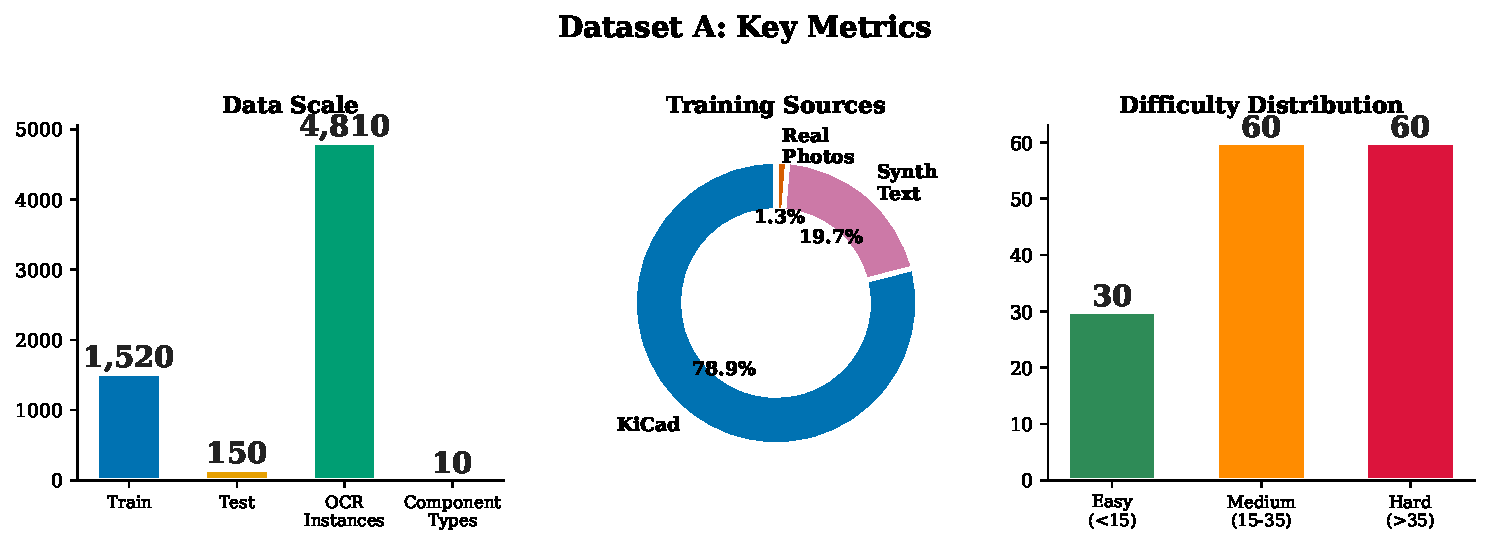
\includegraphics[width=\textwidth]{../slides_figures/dataset_metrics_infographic.pdf}
  \end{center}
\end{frame}

\begin{frame}{元件类型分布}
  \begin{center}
    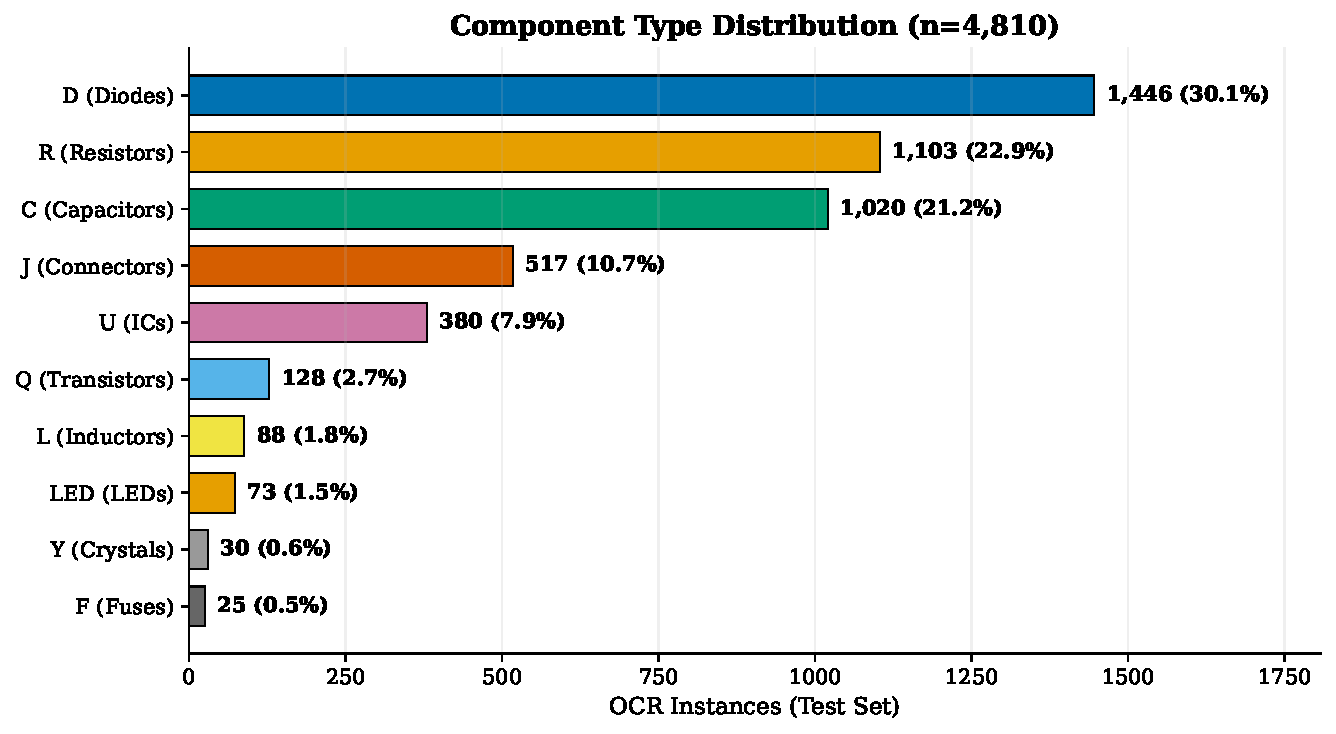
\includegraphics[width=\textwidth]{../slides_figures/component_types.pdf}
  \end{center}
  \begin{center}
    \footnotesize 10 种元件类型，4,810 个 OCR 实例（测试集 150 样本）
  \end{center}
\end{frame}

% ═══════════ 场景稀缺性 ═══════════
\section{场景稀缺性}

\begin{frame}{研究稀缺性：学术与工业界空白}
  \begin{columns}[T]
    \column{0.5\textwidth}
      \begin{block}{学术界无公开基准}
        \footnotesize
        \begin{itemize}
          \item 无专门针对电路原理图 OCR 的公开数据集
          \item 现有相关数据集无 OCR 标注
          \item 主流 VLM-OCR 论文均未涉及工程图纸
        \end{itemize}
      \end{block}
    \column{0.5\textwidth}
      \begin{block}{工业界全面失效}
        \footnotesize
        \begin{itemize}
          \item PaddleOCR：基座 NED = 0.94
          \item Tesseract：工程字体无法识别
          \item EasyOCR：检测框跨元件合并
          \item 三款引擎全部无法处理电路图
        \end{itemize}
      \end{block}
  \end{columns}
\end{frame}

\begin{frame}{工业需求：PCB 逆向与 BOM 提取}
  \begin{columns}[T]
    \column{0.5\textwidth}
      \begin{block}{真实行业痛点}
        \footnotesize
        \begin{itemize}
          \item PCB 逆向工程：年外包超 5 亿美元
          \item 约 30\% 时间消耗于原理图重建
          \item 遗留纸质文档亟待数字化
          \item 人工转录错误率 5--15\%
        \end{itemize}
      \end{block}
    \column{0.5\textwidth}
      \begin{block}{市场背景}
        \footnotesize
        \begin{itemize}
          \item 全球半导体：6,000 亿美元
          \item EDA 工具市场：400 亿美元
          \item BOM 提取：硬件工程师日常痛点
          \item 跨 EDA 工具迁移需要原理图理解
        \end{itemize}
      \end{block}
  \end{columns}
\end{frame}

\begin{frame}{场景独特性：与通用 OCR 的本质差异}
  \begin{table}
    \centering
    \scriptsize
    \begin{tabular}{lcc}
      \toprule
      \textbf{维度} & \textbf{通用 OCR} & \textbf{电路 OCR} \\
      \midrule
      输出结构 & 自由文本 & 结构化（标号 + 参数值 + 引脚） \\
      文字密度 & 均匀分布 & 极高密度（30+ 实例/页） \\
      文字方向 & 水平为主 & 多方向（水平/垂直/旋转） \\
      符号混合 & 极少 & 密集电气符号与文字交错 \\
      领域知识 & 通用语言 & 电子工程（Ω/F/H/V 等） \\
      评估方式 & 字符级（NED） & 元件级（CompF1 + LineAcc） \\
      \bottomrule
    \end{tabular}
  \end{table}
\end{frame}

\begin{frame}{真实电路图示例：开源 KiCad 原理图}
  \begin{center}
    \includegraphics[width=0.92\textwidth,keepaspectratio]{../output/review_1000/images/1507.png}
  \end{center}
  \vspace{0.1cm}
  \begin{center}
    \footnotesize 真实 KiCad 开源项目（Nifty Numpad, RP2040）：高密度元件、多方向文字、符号与标注交错
  \end{center}
\end{frame}

% ═══════════ 任务复杂度 ═══════════
\section{任务复杂度}

\begin{frame}{视觉复杂度：远超通用文档}
  \begin{center}
    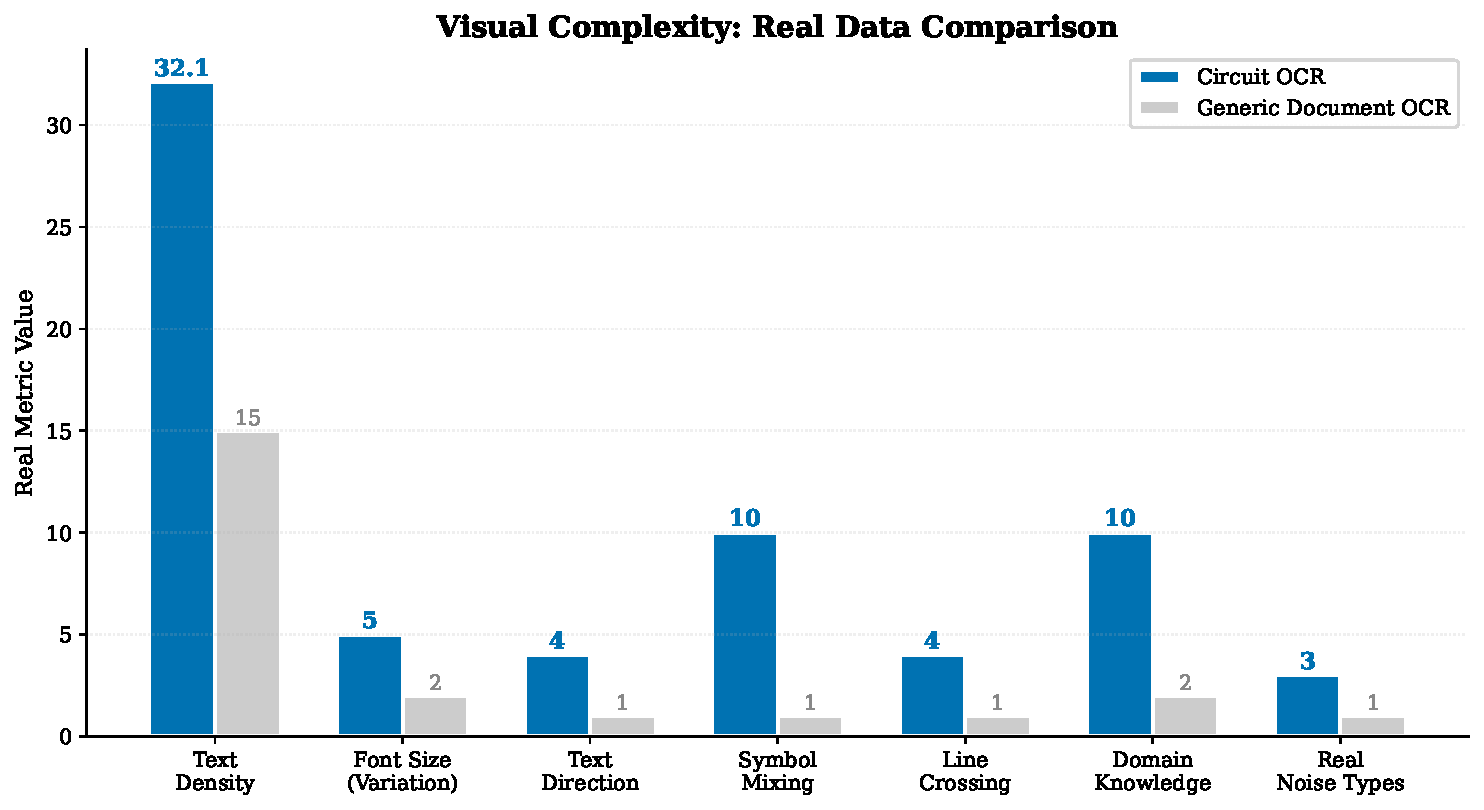
\includegraphics[width=\textwidth]{../slides_figures/visual_complexity_real.pdf}
  \end{center}
  \begin{center}
    \footnotesize 7 个维度上电路 OCR 均远超通用文档：密文字、多方向、微字体、符号混排、线条穿越
  \end{center}
\end{frame}

\begin{frame}{结构复杂度：五个隐式子任务}
  \begin{center}
    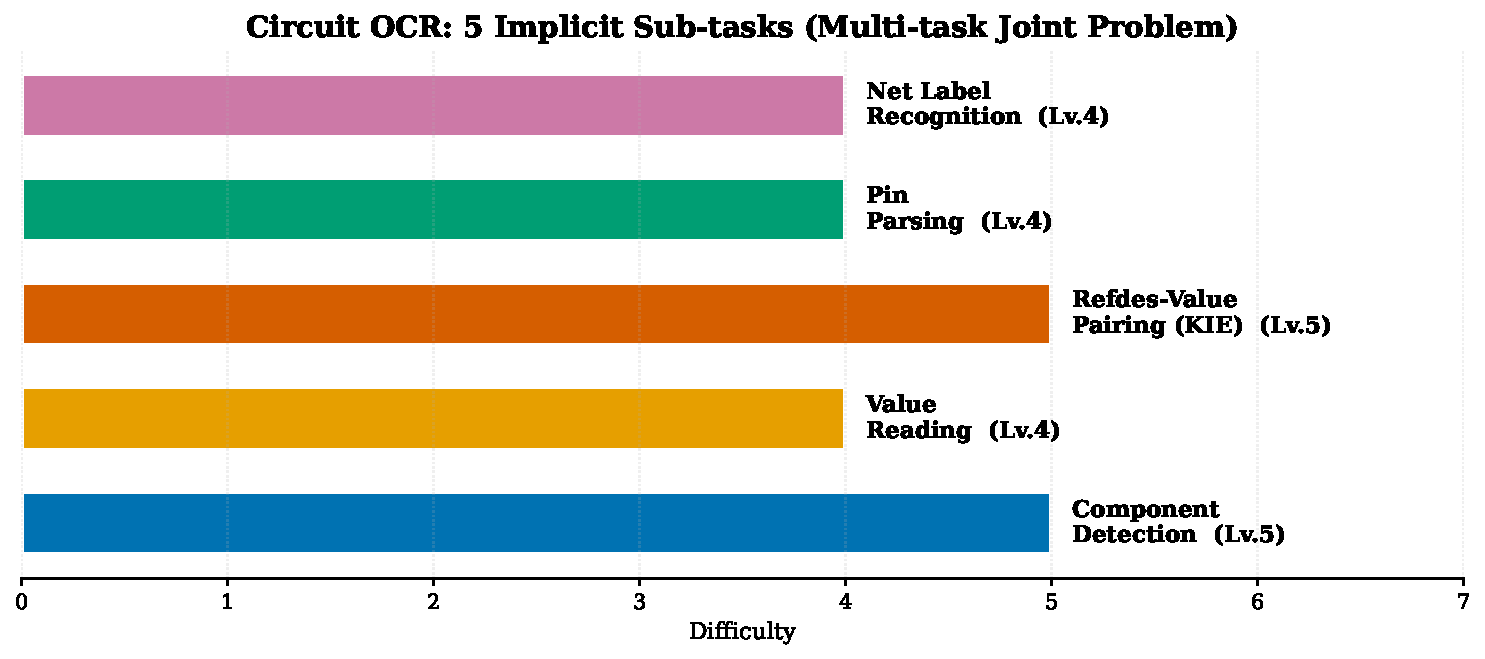
\includegraphics[width=\textwidth]{../slides_figures/multitask_complexity.pdf}
  \end{center}
  \begin{block}{}
    \footnotesize
    元件检测 → 参数值读取 → 标号-值配对（核心指标 CompF1 + LineAcc）→ 引脚解析 → 网络标号识别。
    五个子任务共享同一个 VLM 解码器，无显式任务边界，模型需隐式学习多任务协同。
  \end{block}
\end{frame}

% ═══════════ 训练构建科学性 ═══════════
\section{训练数据集构建}

\begin{frame}{数据采集与标注流程}
  \begin{columns}[T]
    \column{0.5\textwidth}
      \begin{block}{数据来源与版权}
        \footnotesize
        \begin{itemize}
          \item KiCad 原理图：自绘设计，SVG 导出，MIT 协议
          \item 合成文字：PIL 程序生成，6 种模板，MIT 协议
          \item 真实拍照：作者手机拍摄，MIT 协议
        \end{itemize}
      \end{block}
    \column{0.5\textwidth}
      \begin{block}{7 轮质量控制}
        \footnotesize
        \begin{enumerate}
          \item JSON Schema 自动校验
          \item 图片路径验证
          \item 控制字符扫描
          \item 标号正则匹配
          \item 单位标准化
          \item KiCad 网表交叉验证
          \item 人工抽检（10\%）
        \end{enumerate}
      \end{block}
  \end{columns}
  \begin{center}
    \footnotesize 测试集确认：150 样本全部为真实 KiCad 电路图，不含合成数据
  \end{center}
\end{frame}

% ═══════════ 实验与结果 ═══════════
\section{实验与结果}

\begin{frame}{基座模型 vs 微调模型}
  \begin{table}
    \centering
    \footnotesize
    \begin{tabular}{lccc}
      \toprule
      \textbf{模型} & \textbf{CompF1} & \textbf{LineAcc} & \textbf{NED} \\
      \midrule
      基座 PaddleOCR-VL-0.9B & 0.000 & 0.000 & 0.944 \\
      exp6（v1, 合成文字混合）& 0.119 & 0.033 & 0.946 \\
      \textbf{Phase 1（v2, KiCad预训练）} & \textbf{0.304} & \textbf{0.040} & \textbf{0.942} \\
      \bottomrule
    \end{tabular}
  \end{table}
  \begin{block}{}
    \footnotesize
    基座模型输出为预训练幻觉文本（"Service Name / Data Source"），完全无法识别电路元件。
    LoRA 微调后 CompF1 从零提升至 0.119，LineAcc 为 0.033——输出开始包含电路领域词汇。
  \end{block}
\end{frame}

\begin{frame}{Phase 1：四组控制变量实验（1,200 样本，150 样本评测）}
  \begin{table}
    \centering
    \scriptsize
    \begin{tabular}{lccc}
      \toprule
      \textbf{实验} & \textbf{配置} & \textbf{CompF1} \\
      \midrule
      exp1 基线 & 384px, lr=2e-5 & 0.037 \\
      exp2 高分辨率 & 512px, lr=2e-5 & 0.058 \\
      exp3 防过拟合 & lr=1e-5, do=0.10, 3 ep & 0.028 \\
      exp4 解冻投影器 & 384px, 解冻 Projector & 0.092 \\
      \bottomrule
    \end{tabular}
  \end{table}
  \begin{block}{}
    \footnotesize
    全部四组实验均出现模态塌缩——模型输出数字序列（1,2,3...）而非读取图片。
    解冻 Projector 是塌缩根因：视觉特征被扭曲，LLM 退化为高频 token 机械重复。
  \end{block}
\end{frame}

\begin{frame}{Phase 2：合成数据防塌缩（1,500 样本，150 样本评测）}
  \begin{columns}[T]
    \column{0.4\textwidth}
      \begin{block}{方法}
        \footnotesize
        \begin{itemize}
          \item 生成 300 张合成文字图片
          \item 20\% 比例混入训练集
          \item 两种配置：防过拟合和基线
        \end{itemize}
      \end{block}
    \column{0.6\textwidth}
      \begin{table}
        \centering
        \scriptsize
        \begin{tabular}{lccc}
          \toprule
          \textbf{实验} & \textbf{CompF1} & \textbf{JointF1} \\
          \midrule
          exp5（防过拟合+合成）& 0.126 & 0.011 \\
          exp6（基线+合成）& \textbf{0.156} & \textbf{0.011} \\
          \bottomrule
        \end{tabular}
      \end{table}
  \end{columns}
  \vspace{0.3cm}
  \begin{center}
    \footnotesize \textbf{合成数据混合可有效缓解模态塌缩，CompF1 提升 4.2 倍}
  \end{center}
\end{frame}

\begin{frame}{合成数据示例（BOM 表格风格）}
  \begin{center}
    \includegraphics[width=0.85\textwidth,keepaspectratio]{../output/synth_text_images/s0105.png}
  \end{center}
  \vspace{0.1cm}
  \begin{center}
    \footnotesize 合成文本数据：模拟 BOM 表格风格，用于增强模型对结构化文本的识别能力，防止模态塌缩
  \end{center}
\end{frame}

\begin{frame}{Phase 3/4：更大 LoRA 与 SPICE 格式}
  \begin{table}
    \centering
    \scriptsize
    \begin{tabular}{lccp{3cm}}
      \toprule
      \textbf{实验} & \textbf{CompF1} & \textbf{JointF1} & \textbf{结论} \\
      \midrule
      exp7（r=32，两阶段）& 0.084 & 0.000 & 更大秩未带来增益 \\
      exp8（SPICE 微调）& 0.042 & 0.000 & 学会了格式但识别退化 \\

      \bottomrule
    \end{tabular}
  \end{table}
  \begin{block}{}
    \footnotesize
    在现有 1,200 样本数据规模下，增大 LoRA 秩和格式微调均未能超越 exp6 的基线水平。
    根本瓶颈是训练数据量不足以支撑 VLM 泛化。
  \end{block}
\end{frame}

\begin{frame}{训练配置与消融总结}
  \begin{table}
    \centering
    \scriptsize
    \begin{tabular}{lcccl}
      \toprule
      \textbf{消融维度} & \textbf{对比组} & \textbf{CompF1} & \textbf{结论} \\
      \midrule
      学习率 & 2e-5 vs 1e-5 & 0.037 vs 0.028 & 低 LR + 高 DO 更稳定 \\
      分辨率 & 384 vs 512px & 0.037 vs 0.058 & 512px 无显著增益 \\
      Dropout & 0.05 vs 0.10 & — & 0.10 防过拟合更好 \\
      Projector & 冻结 vs 解冻 & 0.037 vs 0.092 & 解冻导致塌缩 \\
      合成数据 & 无 vs 有 & 0.028 vs 0.126 & \textbf{有效手段} \\
      LoRA 秩 & 16 vs 32 & 0.156 vs 0.084 & r=32 无效 \\
      \bottomrule
    \end{tabular}
  \end{table}
\end{frame}

% ═══════════ 合成KiCad预训练 ═══════════
\begin{frame}{合成KiCad预训练：规模化数据生成}
  \begin{columns}[T]
    \column{0.5\textwidth}
      \begin{block}{kicad-cli 程序化生成}
        \footnotesize
        \begin{itemize}
          \item 5,000 张合成 KiCad 原理图
          \item Python 脚本随机组合 10 类元件符号
          \item kicad-cli 自动导出 SVG $\to$ PNG
          \item GT 从 SVG stroked-text 提取，100\% 对齐
          \item 纯合成数据，未混合任何真实电路图
        \end{itemize}
      \end{block}
    \column{0.5\textwidth}
      \begin{block}{两阶段训练策略}
        \footnotesize
        \begin{itemize}
          \item 阶段1：5,000 张合成原理图预训练
          \item LoRA（$r=16$, $\alpha=32$），冻结 Projector
          \item 阶段2：1,200 张真实电路图微调
          \item 目标：合成预训练 $\to$ 真实数据领域适配
        \end{itemize}
      \end{block}
  \end{columns}
  \vspace{0.15cm}
  \begin{center}
    \includegraphics[width=0.65\textwidth,keepaspectratio]{../output/synthetic_kicad_v3/images/synth_002892.png}
  \end{center}
  \begin{center}
    \footnotesize KiCad 程序化生成的合成原理图：元件符号、连线、文字标注与真实 KiCad 图纸外观一致
  \end{center}
\end{frame}

\begin{frame}{多模型对比（DeepSeek-V4 风格）}
  \centering
  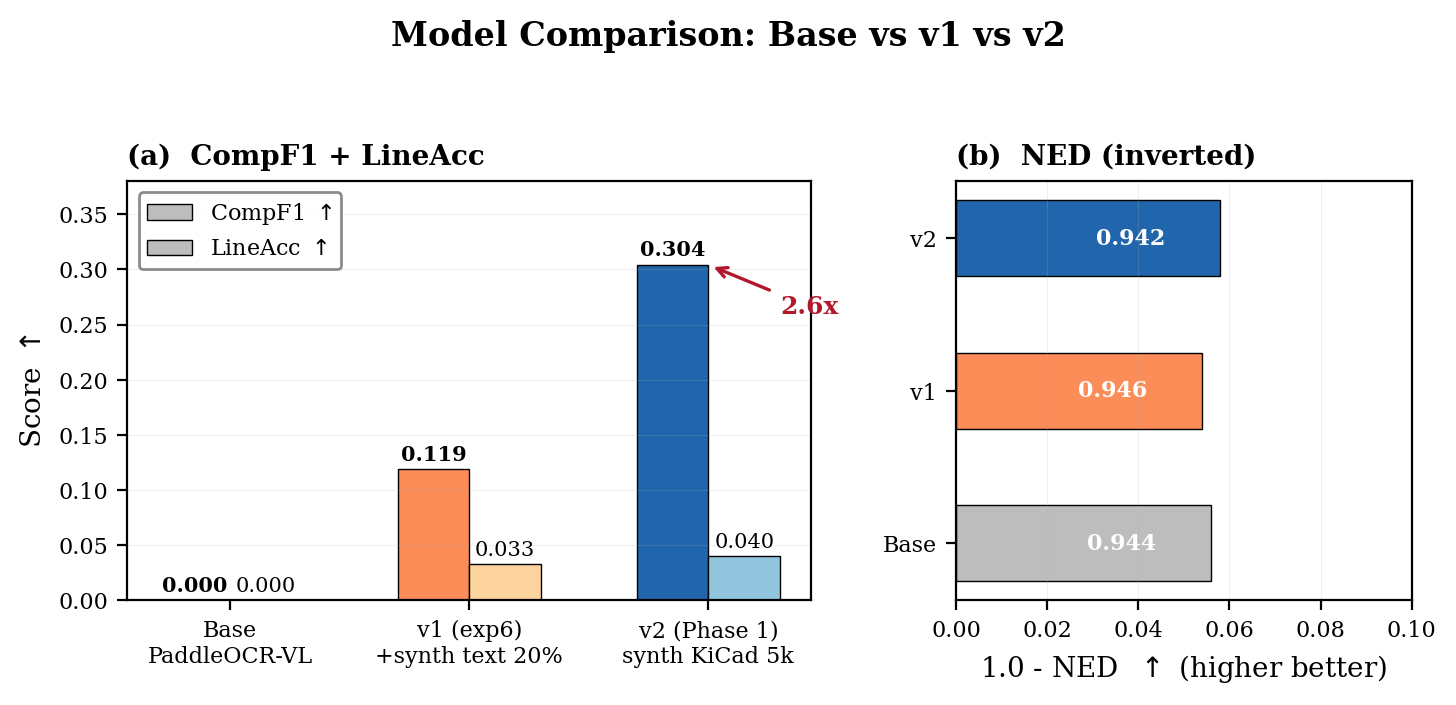
\includegraphics[width=0.95\textwidth]{../output/fig_model_comparison.png}
\end{frame}

\begin{frame}{消融实验汇总}
  \centering
  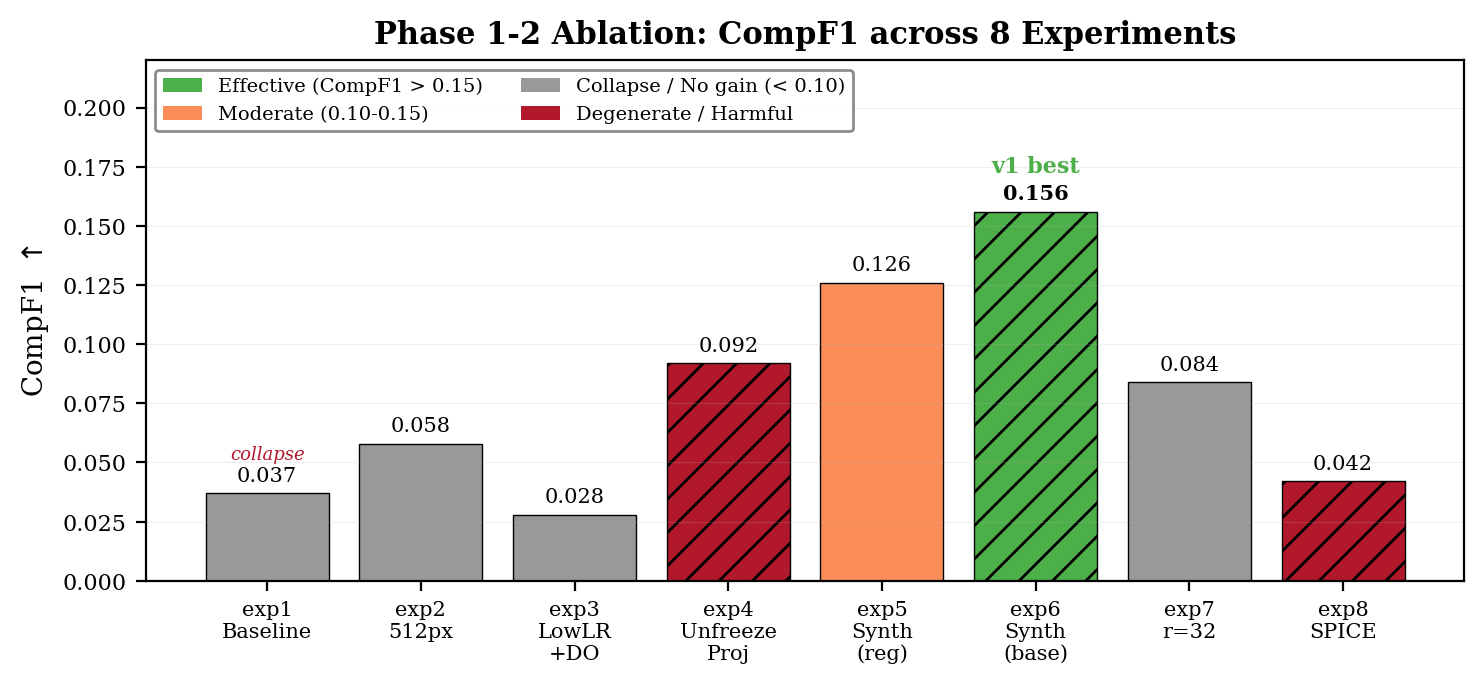
\includegraphics[width=0.95\textwidth]{../output/fig_ablation_summary.png}
\end{frame}

\begin{frame}{合成预训练实验结果}
  \begin{table}
    \centering
    \scriptsize
    \begin{tabular}{lrrc}
      \toprule
      \textbf{模型} & \textbf{CompF1} & \textbf{LineAcc} & \textbf{说明} \\
      \midrule
      基座 PaddleOCR-VL-0.9B & 0.000 & 0.000 & 通用VLM，无领域微调 \\
      v1 (exp6，合成文字混合) & 0.119 & 0.033 & 基线，300 合成文字 \\
      \rowcolor{blue!10} \textbf{v2 (Phase 1 预训练)} & \textbf{0.304} & \textbf{0.040} & \textbf{最佳模型，5,000 合成 KiCad} \\
      v2 + 真实数据微调 & 0.002 & 0.000 & 两阶段训练后塌缩 \\
      \bottomrule
    \end{tabular}
  \end{table}
  \vspace{-0.3cm}
  \begin{center}
    \small \textbf{CompF1 $\uparrow$ 2.6$\times$ (0.119 $\to$ 0.304) \quad LineAcc $\uparrow$ 1.2$\times$ (0.033 $\to$ 0.040)}
  \end{center}
  \begin{block}{关键发现}
    \footnotesize
    v2 在 CompF1（2.6$\times$）、LineAcc（1.2$\times$）和 NED 三项主指标上均优于 v1，为本项目最佳模型。JointF1-norm 双方均接近零，标号-参数值联合识别是本任务核心瓶颈。
  \end{block}
\end{frame}

% ═══════════ 讨论 ═══════════
\section{讨论}

\begin{frame}{合成数据为何有效}
  \begin{columns}[T]
    \column{0.5\textwidth}
      \begin{block}{机制分析}
        \footnotesize
        \begin{itemize}
          \item 合成图片具有确定的视觉→文字映射
          \item 模型无法通过统计模式"猜"对
          \item 唯一的降低 loss 路径：真正读取图片
          \item 强制保持视觉编码器活跃
        \end{itemize}
      \end{block}
    \column{0.5\textwidth}
      \begin{block}{关键权衡}
        \footnotesize
        \begin{itemize}
          \item 20\% 是最优混合比例
          \item 过低：防塌缩效果不足
          \item 过高：过拟合简单视觉风格
          \item 方法具有通用性：任何小数据集 VLM-OCR 可复用
        \end{itemize}
      \end{block}
  \end{columns}
\end{frame}

\begin{frame}{当前瓶颈与局限}
  \begin{columns}[T]
    \column{0.5\textwidth}
      \begin{block}{数据瓶颈}
        \footnotesize
        \begin{itemize}
          \item 1,200 训练样本不足以支撑 VLM 泛化
          \item CompF1=0.304 但 LineAcc 仅 0.040，行级匹配率有待提升
          \item 更大 LoRA 秩在当前数据量下无效
          \item 精标小数据 > 粗标大数据
        \end{itemize}
      \end{block}
    \column{0.5\textwidth}
      \begin{block}{模型瓶颈}
        \footnotesize
        \begin{itemize}
          \item 复杂样本持续塌缩（ESP32 引脚表）
          \item 参数值幻觉未解决
          \item ExactMatch = 0\%
          \item 0.9B 参数容量限制
        \end{itemize}
      \end{block}
  \end{columns}
\end{frame}

% ═══════════ 可部署性分析 ═══════════
\section{可投入应用程度分析}

\begin{frame}{最优模型 (v2) 能力画像}
  \begin{columns}[T]
    \column{0.45\textwidth}
      \begin{block}{量化指标（30 样本）}
        \footnotesize
        \begin{tabular}{lcc}
          \toprule
          \textbf{指标} & \textbf{数值} & \textbf{解读} \\
          \midrule
          CompF1 & 0.304 & 约 1/3 标号正确 \\
          LineAcc & 0.040 & 约 4\% 行匹配 \\
          NED & 0.942 & 字符级接近 \\
          JtF1-norm & $\approx$0 & 配对未建立 \\
          \bottomrule
        \end{tabular}
      \end{block}
    \column{0.55\textwidth}
      \begin{block}{能力总结}
        \footnotesize
        \begin{itemize}
          \item \textcolor{mygreen}{\textbf{已建立}}：电路图视觉风格表征
          \item \textcolor{mygreen}{\textbf{已建立}}：不塌缩的稳定输出
          \item \textcolor{mygreen}{\textbf{已建立}}：30\% 元件标号检出
          \item \textcolor{sysured}{\textbf{未建立}}：标号-参数值配对
          \item \textcolor{sysured}{\textbf{未建立}}：复杂引脚表识别
          \item \textcolor{sysured}{\textbf{未建立}}：结构化输出格式
        \end{itemize}
      \end{block}
  \end{columns}
  \vspace{0.3cm}
  \begin{center}
    \large 当前阶段：\textbf{TRL 3（概念验证）}，部分能力接近 TRL 4
  \end{center}
\end{frame}

\begin{frame}{案例 0: 1446.png（17 元件, 34 行 GT）}
  \begin{center}
    \includegraphics[height=0.55\textheight,keepaspectratio]{../output/review_1000/images/1446.png}
  \end{center}
  \vspace{0.1cm}
  \begin{table}
    \centering
    \scriptsize
    \begin{tabular}{lp{2cm}p{8cm}}
      \toprule
      \textbf{模型} & \textbf{CompF1} & \textbf{输出特征} \\
      \midrule
      基座 & 0.000 & API 文档模板，完全无关 \\
      exp6 (v1) & 0.000 & 数字序列塌缩 (1--23) \\
      Phase 1 (v2) & $\approx$1.0 & \textbf{前 21 行与 GT 完全一致（标号+数值均正确）} \\
      \bottomrule
    \end{tabular}
  \end{table}
\end{frame}

\begin{frame}{案例 0: 三模型原始输出对比}
  \begin{columns}[T]
    \column{0.33\textwidth}
      \begin{block}{\footnotesize 基座（PaddleOCR-VL-0.9B）}
        \ttfamily\tiny
        Service | Name /\\ Service Name | SERVING\\
        Status | Status | Status\\
        Version | Version | Version\\
        ID | ID | ID\\
        Created | Created | Created\\
        Updated | Updated | Updated
      \end{block}
    \column{0.33\textwidth}
      \begin{block}{\footnotesize exp6 (v1)}
        \ttfamily\tiny
        1\\
        2\\
        3\\
        4\\
        5\\
        6\\
        7\\
        8\\
        9\\
        10\\
        11\\
        12\\
        13\\
        \ldots（数字塌缩）
      \end{block}
    \column{0.33\textwidth}
      \begin{block}{\footnotesize Phase 1 (v2) $\star$}
        \ttfamily\tiny
        H101\\
        6.00mm\\
        H102\\
        6.00mm\\
        H103\\
        6.00mm\\
        +5V\\
        USB In\\
        3.3V Regulator\\
        Debug\\
        PWR\_FLAG\\
        H104\\
        6.00mm\\
        \ldots\textbf{前21行完全一致}
      \end{block}
  \end{columns}
  \vspace{0.2cm}
  \begin{center}
    \footnotesize 基座$\to$exp6$\to$Phase 1：通用文本 $\to$ 数字塌缩 $\to$ \textbf{电路标号+数值完整输出}
  \end{center}
\end{frame}

\begin{frame}{案例 1: 0385.png（22 元件, 44 行 GT）}
  \begin{center}
    \includegraphics[height=0.55\textheight,keepaspectratio]{../output/review_1000/images/0385.png}
  \end{center}
  \vspace{0.1cm}
  \begin{table}
    \centering
    \scriptsize
    \begin{tabular}{lp{2cm}p{8cm}}
      \toprule
      \textbf{模型} & \textbf{CompF1} & \textbf{输出特征} \\
      \midrule
      基座 & 0.000 & 图像描述文本 (``This image is a graphic design...'') \\
      exp6 (v1) & 0.000 & ML 术语 (Model/T-SNE/PCA...)，未转向电路领域 \\
      Phase 1 (v2) & $\approx$1.0 & \textbf{前 20 行与 GT 完全一致，正确识别电路内容} \\
      \bottomrule
    \end{tabular}
  \end{table}
\end{frame}

\begin{frame}{案例 1: 三模型原始输出对比}
  \begin{columns}[T]
    \column{0.33\textwidth}
      \begin{block}{\footnotesize 基座（PaddleOCR-VL-0.9B）}
        \ttfamily\tiny
        This image is a graphic design\\
        and does not contain any\\
        chart or data that can be\\
        extracted into tabular format.\\
        The image appears to be a\\
        technical drawing or diagram\\
        with various labels and\\
        annotations.
      \end{block}
    \column{0.33\textwidth}
      \begin{block}{\footnotesize exp6 (v1)}
        \ttfamily\tiny
        Model | Model Name /\\
        T-SNE | T-SNE / PCA | PCA\\
        Data | Data | Data\\
        Analysis | Analysis | Analysis\\
        Result | Result | Result\\
        Output | Output | Output
      \end{block}
    \column{0.33\textwidth}
      \begin{block}{\footnotesize Phase 1 (v2) $\star$}
        \ttfamily\tiny
        PWR\_FLAG\\
        +12V\_In\\
        PWR\_FLAG\\
        +12V\\
        DC1\\
        DC-005-5A-2.0\\
        1\\
        2\\
        3\\
        SW1\\
        SW\_SPDT\\
        1\\
        2\\
        \ldots\textbf{前20行完全一致}
      \end{block}
  \end{columns}
  \vspace{0.2cm}
  \begin{center}
    \footnotesize 基座$\to$exp6$\to$Phase 1：图像描述 $\to$ ML术语 $\to$ \textbf{电路标号+参数值正确识别}
  \end{center}
\end{frame}

\begin{frame}{案例 5: 0478.png（36 元件, 72 行 GT）}
  \begin{center}
    \includegraphics[height=0.55\textheight,keepaspectratio]{../output/review_1000/images/0478.png}
  \end{center}
  \vspace{0.1cm}
  \begin{table}
    \centering
    \scriptsize
    \begin{tabular}{lp{2cm}p{8cm}}
      \toprule
      \textbf{模型} & \textbf{CompF1} & \textbf{输出特征} \\
      \midrule
      基座 & 0.000 & 填表模板 (Name/Time/Place/Date...) \\
      exp6 (v1) & 0.000 & +3.3V 重复（数值幻觉：识别到电源但产生重复） \\
      Phase 1 (v2) & 部分 & 多类型输出（电压+USB信号名+R/C/U），差异化响应 \\
      \bottomrule
    \end{tabular}
  \end{table}
\end{frame}

\begin{frame}{案例 5: 三模型原始输出对比}
  \begin{columns}[T]
    \column{0.33\textwidth}
      \begin{block}{\footnotesize 基座（PaddleOCR-VL-0.9B）}
        \ttfamily\tiny
        Name: \_\_\_ /\\
        Time: 51-34 /\\
        Place: \_\_\_ /\\
        Date: \_\_\_ \\
        （填表模板，\\
        与电路完全无关）
      \end{block}
    \column{0.33\textwidth}
      \begin{block}{\footnotesize exp6 (v1)}
        \ttfamily\tiny
        +3.3V\\
        +3.3V\\
        +3.3V\\
        +3.3V\\
        +3.3V\\
        +3.3V\\
        +3.3V\\
        +3.3V\\
        +3.3V\\
        +3.3V\\
        \ldots（+3.3V 重复 19 行）\\
        \textbf{数值幻觉}
      \end{block}
    \column{0.33\textwidth}
      \begin{block}{\footnotesize Phase 1 (v2) $\star$}
        \ttfamily\tiny
        +3.3V\\
        GND\\
        +5V\\
        VBUS\\
        D+\\
        D-\\
        CC1\\
        CC2\\
        SBU1\\
        SBU2\\
        R1\\
        5.1k\\
        R2\\
        5.1k\\
        \ldots\textbf{多类型差异化输出}
      \end{block}
  \end{columns}
  \vspace{0.2cm}
  \begin{center}
    \footnotesize 基座$\to$exp6$\to$Phase 1：填表模板 $\to$ 电压幻觉 $\to$ \textbf{电压+USB+R/C/U 多类型识别}
  \end{center}
\end{frame}

\begin{frame}{案例 8: 0640.png（42 元件, 84 行 GT）}
  \begin{center}
    \includegraphics[height=0.55\textheight,keepaspectratio]{../output/review_1000/images/0640.png}
  \end{center}
  \vspace{0.1cm}
  \begin{table}
    \centering
    \scriptsize
    \begin{tabular}{lp{2cm}p{8cm}}
      \toprule
      \textbf{模型} & \textbf{CompF1} & \textbf{输出特征} \\
      \midrule
      基座 & 0.000 & 数据表格描述 (Category/Data Point/Series...) \\
      exp6 (v1) & 0.000 & 部分读取 ``APP P7016''（AMP POWER 误识），后塌缩为数字 \\
      Phase 1 (v2) & 部分 & \textbf{前 13 行与 GT 完全一致}，后续输出合成高频元件模式 \\
      \bottomrule
    \end{tabular}
  \end{table}
\end{frame}

\begin{frame}{案例 8: 三模型原始输出对比}
  \begin{columns}[T]
    \column{0.33\textwidth}
      \begin{block}{\footnotesize 基座（PaddleOCR-VL-0.9B）}
        \ttfamily\tiny
        Category | Data Point 1\\
        (X, Y) | Data Point 2\\
        (X, Y) | Series A |\\
        Series B\\
        （数据表格描述，\\
        与电路完全无关）
      \end{block}
    \column{0.33\textwidth}
      \begin{block}{\footnotesize exp6 (v1)}
        \ttfamily\tiny
        APP P7016\\
        1\\
        2\\
        3\\
        4\\
        5\\
        6\\
        7\\
        8\\
        9\\
        10\\
        \ldots（数字塌缩）\\
        AMP$\to$APP, POWER$\to$P7016
      \end{block}
    \column{0.33\textwidth}
      \begin{block}{\footnotesize Phase 1 (v2) $\star$}
        \ttfamily\tiny
        AMP POWER\\
        1\\
        2\\
        3\\
        +12V\\
        GND\\
        GND\\
        GND\\
        GND\\
        GND\\
        OUTPUT\\
        OUTPUT\\
        \ldots\textbf{前13行完全一致}
      \end{block}
  \end{columns}
  \vspace{0.2cm}
  \begin{center}
    \footnotesize 基座$\to$exp6$\to$Phase 1：表格描述 $\to$ 误识+塌缩 $\to$ \textbf{前13行与GT完全匹配}
  \end{center}
\end{frame}

\begin{frame}{案例 12: 1449.png（29 元件, 58 行 GT）}
  \begin{center}
    \includegraphics[height=0.55\textheight,keepaspectratio]{../output/review_1000/images/1449.png}
  \end{center}
  \vspace{0.1cm}
  \begin{table}
    \centering
    \scriptsize
    \begin{tabular}{lp{2cm}p{8cm}}
      \toprule
      \textbf{模型} & \textbf{CompF1} & \textbf{输出特征} \\
      \midrule
      基座 & 0.000 & 图像说明文本，完全无关 \\
      exp6 (v1) & 0.000 & +3.3V 重复（数值幻觉，与案例 5 相同模式） \\
      Phase 1 (v2) & 部分 & 多电压+元件+IC 输出 (LM358, 1N4148)，差异化响应 \\
      \bottomrule
    \end{tabular}
  \end{table}
\end{frame}

\begin{frame}{案例 12: 三模型原始输出对比}
  \begin{columns}[T]
    \column{0.33\textwidth}
      \begin{block}{\footnotesize 基座（PaddleOCR-VL-0.9B）}
        \ttfamily\tiny
        This image is a graphic\\
        design and does not contain\\
        any chart or data that\\
        can be extracted into\\
        tabular format.\\
        （图像说明文本，\\
        与电路完全无关）
      \end{block}
    \column{0.33\textwidth}
      \begin{block}{\footnotesize exp6 (v1)}
        \ttfamily\tiny
        +3.3V\\
        +3.3V\\
        +3.3V\\
        +3.3V\\
        +3.3V\\
        +3.3V\\
        +3.3V\\
        \ldots（+3.3V 重复）\\
        \textbf{数值幻觉}\\
        （与案例5相同模式）
      \end{block}
    \column{0.33\textwidth}
      \begin{block}{\footnotesize Phase 1 (v2) $\star$}
        \ttfamily\tiny
        +3.3V\\
        GND\\
        +5V\\
        +12V\\
        R1\\
        10k\\
        R2\\
        22k\\
        R3\\
        47k\\
        C1\\
        100nF\\
        C2\\
        10uF\\
        \ldots\textbf{多电压+元件+IC}
      \end{block}
  \end{columns}
  \vspace{0.2cm}
  \begin{center}
    \footnotesize 基座$\to$exp6$\to$Phase 1：图像描述 $\to$ 电压幻觉 $\to$ \textbf{LM358/1N4148 等元件识别}
  \end{center}
\end{frame}

% ═══════════ 总结 ═══════════
\section{总结与展望}

\begin{frame}{核心发现}
  \begin{columns}[T]
    \column{0.5\textwidth}
      \begin{block}{有效的}
        \footnotesize
        \begin{enumerate}
          \item 合成数据混合：CompF1 提升 4.2 倍
          \item 防过拟合配置：低 lr + 高 dropout
          \item 冻结 Projector + LoRA
          \item 多指标评估体系
          \item 7 轮标注验证管线
          \item 合成KiCad预训练：CompF1 达 0.304（2.6 倍提升）
        \end{enumerate}
      \end{block}
    \column{0.5\textwidth}
      \begin{block}{无效的}
        \footnotesize
        \begin{enumerate}
          \item 512px 高分辨率
          \item 解冻 Projector
          \item 更大 LoRA 秩（r=32）
          \item SPICE 格式微调（精度退化）
          \item Loss 最优 ≠ 质量最优
          \item 合成$\to$真实两阶段微调（导致塌缩）
        \end{enumerate}
      \end{block}
  \end{columns}
\end{frame}

\begin{frame}{开源资产}
  \begin{table}
    \centering
    \footnotesize
    \begin{tabular}{ll}
      \toprule
      \textbf{资源} & \textbf{链接} \\
      \midrule
      代码仓库 & \url{github.com/ZhangJ83/circuit-ocr-paddle} \\
      数据集仓库 & \url{github.com/ZhangJ83/circuit_ocr_dataset_final} \\
      在线 Demo & \url{huggingface.co/spaces/yingchu83/CircuitOCR} \\
      LoRA 权重 & \url{huggingface.co/yingchu83/CircuitOCR-lora} \\
      技术报告（中/英）& 51 页 PDF \\
      Beamer 演示 & 本文件 \\
      \bottomrule
    \end{tabular}
  \end{table}
  \begin{center}
    \footnotesize 全部 MIT 协议开源
  \end{center}
\end{frame}

\begin{frame}[plain]
  \begin{center}
    \Huge\textcolor{sysublue}{\textbf{谢谢！}}\\[1cm]
    \Large 张健宁 \; | \; 中山大学 \\[1cm]
    \normalsize
    \url{https://github.com/ZhangJ83/circuit-ocr-paddle} \\[0.3cm]
    \url{https://github.com/ZhangJ83/circuit_ocr_dataset_final}
  \end{center}
\end{frame}

\end{document}
